\documentclass[twoside,openright,titlepage,numbers=noenddot,headinclude,%
               footinclude=true,cleardoublepage=empty,abstractoff,BCOR=5mm,%
               paper=a4,fontsize=11pt,ngerman,american]{scrreprt}

% Custom config ===============================================================

% Classic thesis
\usepackage{amssymb}
% ****************************************************************************************************
% classicthesis-config.tex
% formerly known as loadpackages.sty, classicthesis-ldpkg.sty, and classicthesis-preamble.sty
% Use it at the beginning of your ClassicThesis.tex, or as a LaTeX Preamble
% in your ClassicThesis.{tex,lyx} with % ****************************************************************************************************
% classicthesis-config.tex
% formerly known as loadpackages.sty, classicthesis-ldpkg.sty, and classicthesis-preamble.sty
% Use it at the beginning of your ClassicThesis.tex, or as a LaTeX Preamble
% in your ClassicThesis.{tex,lyx} with % ****************************************************************************************************
% classicthesis-config.tex
% formerly known as loadpackages.sty, classicthesis-ldpkg.sty, and classicthesis-preamble.sty
% Use it at the beginning of your ClassicThesis.tex, or as a LaTeX Preamble
% in your ClassicThesis.{tex,lyx} with \input{classicthesis-config}
% ****************************************************************************************************
% If you like the classicthesis, then I would appreciate a postcard.
% My address can be found in the file ClassicThesis.pdf. A collection
% of the postcards I received so far is available online at
% http://postcards.miede.de
% ****************************************************************************************************

% ****************************************************************************************************
% 1. Configure classicthesis for your needs here, e.g., remove "drafting" below
% in order to deactivate the time-stamp on the pages
% ****************************************************************************************************
\PassOptionsToPackage{listings,%drafting,% %eulerchapternumbers,%
				 pdfspacing,eulermath,%floatperchapter,%linedheaders,%
				 subfig,parts,dottedtoc}{classicthesis}
% ********************************************************************
% Available options for classicthesis.sty
% (see ClassicThesis.pdf for more information):
% drafting
% parts nochapters linedheaders
% eulerchapternumbers beramono eulermath pdfspacing minionprospacing
% tocaligned dottedtoc manychapters
% listings floatperchapter subfig
% ********************************************************************

% ********************************************************************
% Triggers for this config
% ********************************************************************
\usepackage{ifthen}
\newboolean{enable-backrefs} % enable backrefs in the bibliography
\setboolean{enable-backrefs}{false} % true false
% ****************************************************************************************************


% ****************************************************************************************************
% 2. Personal data and user ad-hoc commands
% ****************************************************************************************************
\newcommand{\myTitle}{My Title\xspace}
\newcommand{\mySubtitle}{My Subtitle\xspace}
%\newcommand{\myDegree}{Doktor-Ingenieur (Dr.-Ing.)\xspace}
\newcommand{\myName}{Omoju Miller\xspace}
%\newcommand{\myProf}{Put name here\xspace}
%\newcommand{\myOtherProf}{Put name here\xspace}
%\newcommand{\mySupervisor}{Pierre Geurts\xspace}
%\newcommand{\myFaculty}{Faculty of Applied Sciences\xspace}
%\newcommand{\myDepartment}{Department of EE and CS\xspace}
%\newcommand{\myUni}{University of Liege\xspace}
%\newcommand{\myLocation}{Liege, Belgium\xspace}
%\newcommand{\myTime}{June 2014\xspace}
\newcommand{\myVersion}{version 1.0\xspace}

% ********************************************************************
% Setup, finetuning, and useful commands
% ********************************************************************
\newcounter{dummy} % necessary for correct hyperlinks (to index, bib, etc.)
\newlength{\abcd} % for ab..z string length calculation
\providecommand{\mLyX}{L\kern-.1667em\lower.25em\hbox{Y}\kern-.125emX\@}
\newcommand{\ie}{i.\,e.}
\newcommand{\Ie}{I.\,e.}
\newcommand{\eg}{e.\,g.}
\newcommand{\Eg}{E.\,g.}
% ****************************************************************************************************


% ****************************************************************************************************
% 3. Loading some handy packages
% ****************************************************************************************************
% ********************************************************************
% Packages with options that might require adjustments
% ********************************************************************
%\PassOptionsToPackage{latin9}{inputenc}	% latin9 (ISO-8859-9) = latin1+"Euro sign"
% \usepackage{inputenc}

\usepackage[applemac]{inputenc}

%\PassOptionsToPackage{ngerman,american}{babel}   % change this to your language(s)
% Spanish languages need extra options in order to work with this template
%\PassOptionsToPackage{spanish,es-lcroman}{babel}
 \usepackage{babel}

\PassOptionsToPackage{square,authoryear}{natbib}
 \usepackage{natbib}

\PassOptionsToPackage{fleqn}{amsmath}		% math environments and more by the AMS
 \usepackage{amsmath}

% ********************************************************************
% General useful packages
% ********************************************************************
\PassOptionsToPackage{T1}{fontenc} % T2A for cyrillics
	\usepackage{fontenc}


\usepackage{lipsum}
\usepackage{textcomp} % fix warning with missing font shapes
%\usepackage{scrhack} % fix warnings when using KOMA with listings package
\usepackage{xspace} % to get the spacing after macros right
\usepackage{mparhack} % get marginpar right
%\usepackage{fixltx2e} % fixes some LaTeX stuff
\PassOptionsToPackage{printonlyused,smaller}{acronym}
	\usepackage{acronym} % nice macros for handling all acronyms in the thesis
%\renewcommand*{\acsfont}[1]{\textssc{#1}} % for MinionPro
%\renewcommand{\bflabel}[1]{{#1}\hfill} % fix the list of acronyms
% ****************************************************************************************************


% ****************************************************************************************************
% 4. Setup floats: tables, (sub)figures, and captions
% ****************************************************************************************************
\usepackage{tabularx} % better tables
	\setlength{\extrarowheight}{3pt} % increase table row height
\newcommand{\tableheadline}[1]{\multicolumn{1}{c}{\spacedlowsmallcaps{#1}}}
\newcommand{\myfloatalign}{\centering} % to be used with each float for alignment
\usepackage{caption}
\captionsetup{format=hang,font=small}
\usepackage{subfig}
% ****************************************************************************************************


% ****************************************************************************************************
% 5. Setup code listings
% ****************************************************************************************************
\usepackage{listings}
%\lstset{emph={trueIndex,root},emphstyle=\color{BlueViolet}}%\underbar} % for special keywords
\lstset{language=[LaTeX]Tex,%C++,
    keywordstyle=\color{RoyalBlue},%\bfseries,
    basicstyle=\small\ttfamily,
    %identifierstyle=\color{NavyBlue},
    commentstyle=\color{Green}\ttfamily,
    stringstyle=\rmfamily,
    numbers=none,%left,%
    numberstyle=\scriptsize,%\tiny
    stepnumber=5,
    numbersep=8pt,
    showstringspaces=false,
    breaklines=true,
    frameround=ftff,
    frame=single,
    belowcaptionskip=.75\baselineskip
    %frame=L
}
% ****************************************************************************************************


% ****************************************************************************************************
% 6. PDFLaTeX, hyperreferences and citation backreferences
% ****************************************************************************************************
% ********************************************************************
% Using PDFLaTeX
% ********************************************************************
\PassOptionsToPackage{pdftex,hyperfootnotes=true,pdfpagelabels}{hyperref}
	\usepackage{hyperref}  % backref linktocpage pagebackref
\pdfcompresslevel=9
\pdfadjustspacing=1
\PassOptionsToPackage{pdftex}{graphicx}
	\usepackage{graphicx}

% ********************************************************************
% Setup the style of the backrefs from the bibliography
% (translate the options to any language you use)
% ********************************************************************
\newcommand{\backrefnotcitedstring}{\relax}%(Not cited.)
\newcommand{\backrefcitedsinglestring}[1]{(Cited on page~#1.)}
\newcommand{\backrefcitedmultistring}[1]{(Cited on pages~#1.)}
\ifthenelse{\boolean{enable-backrefs}}%
{%
		\PassOptionsToPackage{hyperpageref}{backref}
		\usepackage{backref} % to be loaded after hyperref package
		   \renewcommand{\backreftwosep}{ and~} % separate 2 pages
		   \renewcommand{\backreflastsep}{, and~} % separate last of longer list
		   \renewcommand*{\backref}[1]{}  % disable standard
		   \renewcommand*{\backrefalt}[4]{% detailed backref
		      \ifcase #1 %
		         \backrefnotcitedstring%
		      \or%
		         \backrefcitedsinglestring{#2}%
		      \else%
		         \backrefcitedmultistring{#2}%
		      \fi}%
}{\relax}

% ********************************************************************
% Hyperreferences
% ********************************************************************
\hypersetup{%
    %draft,	% = no hyperlinking at all (useful in b/w printouts)
    colorlinks=true, linktocpage=true, pdfstartpage=3, pdfstartview=FitV,%
    % uncomment the following line if you want to have black links (e.g., for printing)
    %colorlinks=false, linktocpage=false, pdfborder={0 0 0}, pdfstartpage=3, pdfstartview=FitV,%
    breaklinks=true, pdfpagemode=UseNone, pageanchor=true, pdfpagemode=UseOutlines,%
    plainpages=false, bookmarksnumbered, bookmarksopen=true, bookmarksopenlevel=1,%
    hypertexnames=true, pdfhighlight=/O,%nesting=true,%frenchlinks,%
    urlcolor=webbrown, linkcolor=RoyalBlue, citecolor=webgreen, %pagecolor=RoyalBlue,%
    %urlcolor=Black, linkcolor=Black, citecolor=Black, %pagecolor=Black,%
    pdftitle={\myTitle},%
    pdfauthor={\textcopyright\ \myName},%
    pdfsubject={},%
    pdfkeywords={},%
    pdfcreator={pdfLaTeX},%
    pdfproducer={LaTeX with hyperref and classicthesis}%
}

% ********************************************************************
% Setup autoreferences
% ********************************************************************
% There are some issues regarding autorefnames
% http://www.ureader.de/msg/136221647.aspx
% http://www.tex.ac.uk/cgi-bin/texfaq2html?label=latexwords
% you have to redefine the makros for the
% language you use, e.g., american, ngerman
% (as chosen when loading babel/AtBeginDocument)
% ********************************************************************
\makeatletter
\@ifpackageloaded{babel}%
    {%
       \addto\extrasamerican{%
					\renewcommand*{\figureautorefname}{Figure}%
					\renewcommand*{\tableautorefname}{Table}%
					\renewcommand*{\partautorefname}{Part}%
					\renewcommand*{\chapterautorefname}{Chapter}%
					\renewcommand*{\sectionautorefname}{Section}%
					\renewcommand*{\subsectionautorefname}{Section}%
					\renewcommand*{\subsubsectionautorefname}{Section}%
				}%
       \addto\extrasngerman{%
					\renewcommand*{\paragraphautorefname}{Absatz}%
					\renewcommand*{\subparagraphautorefname}{Unterabsatz}%
					\renewcommand*{\footnoteautorefname}{Fu\"snote}%
					\renewcommand*{\FancyVerbLineautorefname}{Zeile}%
					\renewcommand*{\theoremautorefname}{Theorem}%
					\renewcommand*{\appendixautorefname}{Anhang}%
					\renewcommand*{\equationautorefname}{Gleichung}%
					\renewcommand*{\itemautorefname}{Punkt}%
				}%
			% Fix to getting autorefs for subfigures right (thanks to Belinda Vogt for changing the definition)
			\providecommand{\subfigureautorefname}{\figureautorefname}%
    }{\relax}
\makeatother


% ****************************************************************************************************
% 7. Last calls before the bar closes
% ****************************************************************************************************
% ********************************************************************
% Development Stuff
% ********************************************************************
\listfiles
%\PassOptionsToPackage{l2tabu,orthodox,abort}{nag}
%	\usepackage{nag}
%\PassOptionsToPackage{warning, all}{onlyamsmath}
%	\usepackage{onlyamsmath}

% ********************************************************************
% Last, but not least...
% ********************************************************************
\usepackage{classicthesis}
% ****************************************************************************************************


% ****************************************************************************************************
% 8. Further adjustments (experimental)
% ****************************************************************************************************
% ********************************************************************
% Changing the text area
% ********************************************************************
%\linespread{1.05} % a bit more for Palatino
%\areaset[current]{312pt}{761pt} % 686 (factor 2.2) + 33 head + 42 head \the\footskip
%\setlength{\marginparwidth}{7em}%
%\setlength{\marginparsep}{2em}%

% ********************************************************************
% Using different fonts
% ********************************************************************
%\usepackage[oldstylenums]{kpfonts} % oldstyle notextcomp
%\usepackage[osf]{libertine}
%\usepackage{hfoldsty} % Computer Modern with osf
%\usepackage[light,condensed,math]{iwona}
%\renewcommand{\sfdefault}{iwona}
%\usepackage{lmodern} % <-- no osf support :-(
% \usepackage[T1]{fontenc}
% \usepackage{textcomp}
%\usepackage[urw-garamond]{mathdesign} <-- no osf support :-(
% ****************************************************************************************************

% ****************************************************************************************************
% If you like the classicthesis, then I would appreciate a postcard.
% My address can be found in the file ClassicThesis.pdf. A collection
% of the postcards I received so far is available online at
% http://postcards.miede.de
% ****************************************************************************************************

% ****************************************************************************************************
% 1. Configure classicthesis for your needs here, e.g., remove "drafting" below
% in order to deactivate the time-stamp on the pages
% ****************************************************************************************************
\PassOptionsToPackage{listings,%drafting,% %eulerchapternumbers,%
				 pdfspacing,eulermath,%floatperchapter,%linedheaders,%
				 subfig,parts,dottedtoc}{classicthesis}
% ********************************************************************
% Available options for classicthesis.sty
% (see ClassicThesis.pdf for more information):
% drafting
% parts nochapters linedheaders
% eulerchapternumbers beramono eulermath pdfspacing minionprospacing
% tocaligned dottedtoc manychapters
% listings floatperchapter subfig
% ********************************************************************

% ********************************************************************
% Triggers for this config
% ********************************************************************
\usepackage{ifthen}
\newboolean{enable-backrefs} % enable backrefs in the bibliography
\setboolean{enable-backrefs}{false} % true false
% ****************************************************************************************************


% ****************************************************************************************************
% 2. Personal data and user ad-hoc commands
% ****************************************************************************************************
\newcommand{\myTitle}{My Title\xspace}
\newcommand{\mySubtitle}{My Subtitle\xspace}
%\newcommand{\myDegree}{Doktor-Ingenieur (Dr.-Ing.)\xspace}
\newcommand{\myName}{Omoju Miller\xspace}
%\newcommand{\myProf}{Put name here\xspace}
%\newcommand{\myOtherProf}{Put name here\xspace}
%\newcommand{\mySupervisor}{Pierre Geurts\xspace}
%\newcommand{\myFaculty}{Faculty of Applied Sciences\xspace}
%\newcommand{\myDepartment}{Department of EE and CS\xspace}
%\newcommand{\myUni}{University of Liege\xspace}
%\newcommand{\myLocation}{Liege, Belgium\xspace}
%\newcommand{\myTime}{June 2014\xspace}
\newcommand{\myVersion}{version 1.0\xspace}

% ********************************************************************
% Setup, finetuning, and useful commands
% ********************************************************************
\newcounter{dummy} % necessary for correct hyperlinks (to index, bib, etc.)
\newlength{\abcd} % for ab..z string length calculation
\providecommand{\mLyX}{L\kern-.1667em\lower.25em\hbox{Y}\kern-.125emX\@}
\newcommand{\ie}{i.\,e.}
\newcommand{\Ie}{I.\,e.}
\newcommand{\eg}{e.\,g.}
\newcommand{\Eg}{E.\,g.}
% ****************************************************************************************************


% ****************************************************************************************************
% 3. Loading some handy packages
% ****************************************************************************************************
% ********************************************************************
% Packages with options that might require adjustments
% ********************************************************************
%\PassOptionsToPackage{latin9}{inputenc}	% latin9 (ISO-8859-9) = latin1+"Euro sign"
% \usepackage{inputenc}

\usepackage[applemac]{inputenc}

%\PassOptionsToPackage{ngerman,american}{babel}   % change this to your language(s)
% Spanish languages need extra options in order to work with this template
%\PassOptionsToPackage{spanish,es-lcroman}{babel}
 \usepackage{babel}

\PassOptionsToPackage{square,authoryear}{natbib}
 \usepackage{natbib}

\PassOptionsToPackage{fleqn}{amsmath}		% math environments and more by the AMS
 \usepackage{amsmath}

% ********************************************************************
% General useful packages
% ********************************************************************
\PassOptionsToPackage{T1}{fontenc} % T2A for cyrillics
	\usepackage{fontenc}


\usepackage{lipsum}
\usepackage{textcomp} % fix warning with missing font shapes
%\usepackage{scrhack} % fix warnings when using KOMA with listings package
\usepackage{xspace} % to get the spacing after macros right
\usepackage{mparhack} % get marginpar right
%\usepackage{fixltx2e} % fixes some LaTeX stuff
\PassOptionsToPackage{printonlyused,smaller}{acronym}
	\usepackage{acronym} % nice macros for handling all acronyms in the thesis
%\renewcommand*{\acsfont}[1]{\textssc{#1}} % for MinionPro
%\renewcommand{\bflabel}[1]{{#1}\hfill} % fix the list of acronyms
% ****************************************************************************************************


% ****************************************************************************************************
% 4. Setup floats: tables, (sub)figures, and captions
% ****************************************************************************************************
\usepackage{tabularx} % better tables
	\setlength{\extrarowheight}{3pt} % increase table row height
\newcommand{\tableheadline}[1]{\multicolumn{1}{c}{\spacedlowsmallcaps{#1}}}
\newcommand{\myfloatalign}{\centering} % to be used with each float for alignment
\usepackage{caption}
\captionsetup{format=hang,font=small}
\usepackage{subfig}
% ****************************************************************************************************


% ****************************************************************************************************
% 5. Setup code listings
% ****************************************************************************************************
\usepackage{listings}
%\lstset{emph={trueIndex,root},emphstyle=\color{BlueViolet}}%\underbar} % for special keywords
\lstset{language=[LaTeX]Tex,%C++,
    keywordstyle=\color{RoyalBlue},%\bfseries,
    basicstyle=\small\ttfamily,
    %identifierstyle=\color{NavyBlue},
    commentstyle=\color{Green}\ttfamily,
    stringstyle=\rmfamily,
    numbers=none,%left,%
    numberstyle=\scriptsize,%\tiny
    stepnumber=5,
    numbersep=8pt,
    showstringspaces=false,
    breaklines=true,
    frameround=ftff,
    frame=single,
    belowcaptionskip=.75\baselineskip
    %frame=L
}
% ****************************************************************************************************


% ****************************************************************************************************
% 6. PDFLaTeX, hyperreferences and citation backreferences
% ****************************************************************************************************
% ********************************************************************
% Using PDFLaTeX
% ********************************************************************
\PassOptionsToPackage{pdftex,hyperfootnotes=true,pdfpagelabels}{hyperref}
	\usepackage{hyperref}  % backref linktocpage pagebackref
\pdfcompresslevel=9
\pdfadjustspacing=1
\PassOptionsToPackage{pdftex}{graphicx}
	\usepackage{graphicx}

% ********************************************************************
% Setup the style of the backrefs from the bibliography
% (translate the options to any language you use)
% ********************************************************************
\newcommand{\backrefnotcitedstring}{\relax}%(Not cited.)
\newcommand{\backrefcitedsinglestring}[1]{(Cited on page~#1.)}
\newcommand{\backrefcitedmultistring}[1]{(Cited on pages~#1.)}
\ifthenelse{\boolean{enable-backrefs}}%
{%
		\PassOptionsToPackage{hyperpageref}{backref}
		\usepackage{backref} % to be loaded after hyperref package
		   \renewcommand{\backreftwosep}{ and~} % separate 2 pages
		   \renewcommand{\backreflastsep}{, and~} % separate last of longer list
		   \renewcommand*{\backref}[1]{}  % disable standard
		   \renewcommand*{\backrefalt}[4]{% detailed backref
		      \ifcase #1 %
		         \backrefnotcitedstring%
		      \or%
		         \backrefcitedsinglestring{#2}%
		      \else%
		         \backrefcitedmultistring{#2}%
		      \fi}%
}{\relax}

% ********************************************************************
% Hyperreferences
% ********************************************************************
\hypersetup{%
    %draft,	% = no hyperlinking at all (useful in b/w printouts)
    colorlinks=true, linktocpage=true, pdfstartpage=3, pdfstartview=FitV,%
    % uncomment the following line if you want to have black links (e.g., for printing)
    %colorlinks=false, linktocpage=false, pdfborder={0 0 0}, pdfstartpage=3, pdfstartview=FitV,%
    breaklinks=true, pdfpagemode=UseNone, pageanchor=true, pdfpagemode=UseOutlines,%
    plainpages=false, bookmarksnumbered, bookmarksopen=true, bookmarksopenlevel=1,%
    hypertexnames=true, pdfhighlight=/O,%nesting=true,%frenchlinks,%
    urlcolor=webbrown, linkcolor=RoyalBlue, citecolor=webgreen, %pagecolor=RoyalBlue,%
    %urlcolor=Black, linkcolor=Black, citecolor=Black, %pagecolor=Black,%
    pdftitle={\myTitle},%
    pdfauthor={\textcopyright\ \myName},%
    pdfsubject={},%
    pdfkeywords={},%
    pdfcreator={pdfLaTeX},%
    pdfproducer={LaTeX with hyperref and classicthesis}%
}

% ********************************************************************
% Setup autoreferences
% ********************************************************************
% There are some issues regarding autorefnames
% http://www.ureader.de/msg/136221647.aspx
% http://www.tex.ac.uk/cgi-bin/texfaq2html?label=latexwords
% you have to redefine the makros for the
% language you use, e.g., american, ngerman
% (as chosen when loading babel/AtBeginDocument)
% ********************************************************************
\makeatletter
\@ifpackageloaded{babel}%
    {%
       \addto\extrasamerican{%
					\renewcommand*{\figureautorefname}{Figure}%
					\renewcommand*{\tableautorefname}{Table}%
					\renewcommand*{\partautorefname}{Part}%
					\renewcommand*{\chapterautorefname}{Chapter}%
					\renewcommand*{\sectionautorefname}{Section}%
					\renewcommand*{\subsectionautorefname}{Section}%
					\renewcommand*{\subsubsectionautorefname}{Section}%
				}%
       \addto\extrasngerman{%
					\renewcommand*{\paragraphautorefname}{Absatz}%
					\renewcommand*{\subparagraphautorefname}{Unterabsatz}%
					\renewcommand*{\footnoteautorefname}{Fu\"snote}%
					\renewcommand*{\FancyVerbLineautorefname}{Zeile}%
					\renewcommand*{\theoremautorefname}{Theorem}%
					\renewcommand*{\appendixautorefname}{Anhang}%
					\renewcommand*{\equationautorefname}{Gleichung}%
					\renewcommand*{\itemautorefname}{Punkt}%
				}%
			% Fix to getting autorefs for subfigures right (thanks to Belinda Vogt for changing the definition)
			\providecommand{\subfigureautorefname}{\figureautorefname}%
    }{\relax}
\makeatother


% ****************************************************************************************************
% 7. Last calls before the bar closes
% ****************************************************************************************************
% ********************************************************************
% Development Stuff
% ********************************************************************
\listfiles
%\PassOptionsToPackage{l2tabu,orthodox,abort}{nag}
%	\usepackage{nag}
%\PassOptionsToPackage{warning, all}{onlyamsmath}
%	\usepackage{onlyamsmath}

% ********************************************************************
% Last, but not least...
% ********************************************************************
\usepackage{classicthesis}
% ****************************************************************************************************


% ****************************************************************************************************
% 8. Further adjustments (experimental)
% ****************************************************************************************************
% ********************************************************************
% Changing the text area
% ********************************************************************
%\linespread{1.05} % a bit more for Palatino
%\areaset[current]{312pt}{761pt} % 686 (factor 2.2) + 33 head + 42 head \the\footskip
%\setlength{\marginparwidth}{7em}%
%\setlength{\marginparsep}{2em}%

% ********************************************************************
% Using different fonts
% ********************************************************************
%\usepackage[oldstylenums]{kpfonts} % oldstyle notextcomp
%\usepackage[osf]{libertine}
%\usepackage{hfoldsty} % Computer Modern with osf
%\usepackage[light,condensed,math]{iwona}
%\renewcommand{\sfdefault}{iwona}
%\usepackage{lmodern} % <-- no osf support :-(
% \usepackage[T1]{fontenc}
% \usepackage{textcomp}
%\usepackage[urw-garamond]{mathdesign} <-- no osf support :-(
% ****************************************************************************************************

% ****************************************************************************************************
% If you like the classicthesis, then I would appreciate a postcard.
% My address can be found in the file ClassicThesis.pdf. A collection
% of the postcards I received so far is available online at
% http://postcards.miede.de
% ****************************************************************************************************

% ****************************************************************************************************
% 1. Configure classicthesis for your needs here, e.g., remove "drafting" below
% in order to deactivate the time-stamp on the pages
% ****************************************************************************************************
\PassOptionsToPackage{listings,%drafting,% %eulerchapternumbers,%
				 pdfspacing,eulermath,%floatperchapter,%linedheaders,%
				 subfig,parts,dottedtoc}{classicthesis}
% ********************************************************************
% Available options for classicthesis.sty
% (see ClassicThesis.pdf for more information):
% drafting
% parts nochapters linedheaders
% eulerchapternumbers beramono eulermath pdfspacing minionprospacing
% tocaligned dottedtoc manychapters
% listings floatperchapter subfig
% ********************************************************************

% ********************************************************************
% Triggers for this config
% ********************************************************************
\usepackage{ifthen}
\newboolean{enable-backrefs} % enable backrefs in the bibliography
\setboolean{enable-backrefs}{false} % true false
% ****************************************************************************************************


% ****************************************************************************************************
% 2. Personal data and user ad-hoc commands
% ****************************************************************************************************
\newcommand{\myTitle}{My Title\xspace}
\newcommand{\mySubtitle}{My Subtitle\xspace}
%\newcommand{\myDegree}{Doktor-Ingenieur (Dr.-Ing.)\xspace}
\newcommand{\myName}{Omoju Miller\xspace}
%\newcommand{\myProf}{Put name here\xspace}
%\newcommand{\myOtherProf}{Put name here\xspace}
%\newcommand{\mySupervisor}{Pierre Geurts\xspace}
%\newcommand{\myFaculty}{Faculty of Applied Sciences\xspace}
%\newcommand{\myDepartment}{Department of EE and CS\xspace}
%\newcommand{\myUni}{University of Liege\xspace}
%\newcommand{\myLocation}{Liege, Belgium\xspace}
%\newcommand{\myTime}{June 2014\xspace}
\newcommand{\myVersion}{version 1.0\xspace}

% ********************************************************************
% Setup, finetuning, and useful commands
% ********************************************************************
\newcounter{dummy} % necessary for correct hyperlinks (to index, bib, etc.)
\newlength{\abcd} % for ab..z string length calculation
\providecommand{\mLyX}{L\kern-.1667em\lower.25em\hbox{Y}\kern-.125emX\@}
\newcommand{\ie}{i.\,e.}
\newcommand{\Ie}{I.\,e.}
\newcommand{\eg}{e.\,g.}
\newcommand{\Eg}{E.\,g.}
% ****************************************************************************************************


% ****************************************************************************************************
% 3. Loading some handy packages
% ****************************************************************************************************
% ********************************************************************
% Packages with options that might require adjustments
% ********************************************************************
%\PassOptionsToPackage{latin9}{inputenc}	% latin9 (ISO-8859-9) = latin1+"Euro sign"
% \usepackage{inputenc}

\usepackage[applemac]{inputenc}

%\PassOptionsToPackage{ngerman,american}{babel}   % change this to your language(s)
% Spanish languages need extra options in order to work with this template
%\PassOptionsToPackage{spanish,es-lcroman}{babel}
 \usepackage{babel}

\PassOptionsToPackage{square,authoryear}{natbib}
 \usepackage{natbib}

\PassOptionsToPackage{fleqn}{amsmath}		% math environments and more by the AMS
 \usepackage{amsmath}

% ********************************************************************
% General useful packages
% ********************************************************************
\PassOptionsToPackage{T1}{fontenc} % T2A for cyrillics
	\usepackage{fontenc}


\usepackage{lipsum}
\usepackage{textcomp} % fix warning with missing font shapes
%\usepackage{scrhack} % fix warnings when using KOMA with listings package
\usepackage{xspace} % to get the spacing after macros right
\usepackage{mparhack} % get marginpar right
%\usepackage{fixltx2e} % fixes some LaTeX stuff
\PassOptionsToPackage{printonlyused,smaller}{acronym}
	\usepackage{acronym} % nice macros for handling all acronyms in the thesis
%\renewcommand*{\acsfont}[1]{\textssc{#1}} % for MinionPro
%\renewcommand{\bflabel}[1]{{#1}\hfill} % fix the list of acronyms
% ****************************************************************************************************


% ****************************************************************************************************
% 4. Setup floats: tables, (sub)figures, and captions
% ****************************************************************************************************
\usepackage{tabularx} % better tables
	\setlength{\extrarowheight}{3pt} % increase table row height
\newcommand{\tableheadline}[1]{\multicolumn{1}{c}{\spacedlowsmallcaps{#1}}}
\newcommand{\myfloatalign}{\centering} % to be used with each float for alignment
\usepackage{caption}
\captionsetup{format=hang,font=small}
\usepackage{subfig}
% ****************************************************************************************************


% ****************************************************************************************************
% 5. Setup code listings
% ****************************************************************************************************
\usepackage{listings}
%\lstset{emph={trueIndex,root},emphstyle=\color{BlueViolet}}%\underbar} % for special keywords
\lstset{language=[LaTeX]Tex,%C++,
    keywordstyle=\color{RoyalBlue},%\bfseries,
    basicstyle=\small\ttfamily,
    %identifierstyle=\color{NavyBlue},
    commentstyle=\color{Green}\ttfamily,
    stringstyle=\rmfamily,
    numbers=none,%left,%
    numberstyle=\scriptsize,%\tiny
    stepnumber=5,
    numbersep=8pt,
    showstringspaces=false,
    breaklines=true,
    frameround=ftff,
    frame=single,
    belowcaptionskip=.75\baselineskip
    %frame=L
}
% ****************************************************************************************************


% ****************************************************************************************************
% 6. PDFLaTeX, hyperreferences and citation backreferences
% ****************************************************************************************************
% ********************************************************************
% Using PDFLaTeX
% ********************************************************************
\PassOptionsToPackage{pdftex,hyperfootnotes=true,pdfpagelabels}{hyperref}
	\usepackage{hyperref}  % backref linktocpage pagebackref
\pdfcompresslevel=9
\pdfadjustspacing=1
\PassOptionsToPackage{pdftex}{graphicx}
	\usepackage{graphicx}

% ********************************************************************
% Setup the style of the backrefs from the bibliography
% (translate the options to any language you use)
% ********************************************************************
\newcommand{\backrefnotcitedstring}{\relax}%(Not cited.)
\newcommand{\backrefcitedsinglestring}[1]{(Cited on page~#1.)}
\newcommand{\backrefcitedmultistring}[1]{(Cited on pages~#1.)}
\ifthenelse{\boolean{enable-backrefs}}%
{%
		\PassOptionsToPackage{hyperpageref}{backref}
		\usepackage{backref} % to be loaded after hyperref package
		   \renewcommand{\backreftwosep}{ and~} % separate 2 pages
		   \renewcommand{\backreflastsep}{, and~} % separate last of longer list
		   \renewcommand*{\backref}[1]{}  % disable standard
		   \renewcommand*{\backrefalt}[4]{% detailed backref
		      \ifcase #1 %
		         \backrefnotcitedstring%
		      \or%
		         \backrefcitedsinglestring{#2}%
		      \else%
		         \backrefcitedmultistring{#2}%
		      \fi}%
}{\relax}

% ********************************************************************
% Hyperreferences
% ********************************************************************
\hypersetup{%
    %draft,	% = no hyperlinking at all (useful in b/w printouts)
    colorlinks=true, linktocpage=true, pdfstartpage=3, pdfstartview=FitV,%
    % uncomment the following line if you want to have black links (e.g., for printing)
    %colorlinks=false, linktocpage=false, pdfborder={0 0 0}, pdfstartpage=3, pdfstartview=FitV,%
    breaklinks=true, pdfpagemode=UseNone, pageanchor=true, pdfpagemode=UseOutlines,%
    plainpages=false, bookmarksnumbered, bookmarksopen=true, bookmarksopenlevel=1,%
    hypertexnames=true, pdfhighlight=/O,%nesting=true,%frenchlinks,%
    urlcolor=webbrown, linkcolor=RoyalBlue, citecolor=webgreen, %pagecolor=RoyalBlue,%
    %urlcolor=Black, linkcolor=Black, citecolor=Black, %pagecolor=Black,%
    pdftitle={\myTitle},%
    pdfauthor={\textcopyright\ \myName},%
    pdfsubject={},%
    pdfkeywords={},%
    pdfcreator={pdfLaTeX},%
    pdfproducer={LaTeX with hyperref and classicthesis}%
}

% ********************************************************************
% Setup autoreferences
% ********************************************************************
% There are some issues regarding autorefnames
% http://www.ureader.de/msg/136221647.aspx
% http://www.tex.ac.uk/cgi-bin/texfaq2html?label=latexwords
% you have to redefine the makros for the
% language you use, e.g., american, ngerman
% (as chosen when loading babel/AtBeginDocument)
% ********************************************************************
\makeatletter
\@ifpackageloaded{babel}%
    {%
       \addto\extrasamerican{%
					\renewcommand*{\figureautorefname}{Figure}%
					\renewcommand*{\tableautorefname}{Table}%
					\renewcommand*{\partautorefname}{Part}%
					\renewcommand*{\chapterautorefname}{Chapter}%
					\renewcommand*{\sectionautorefname}{Section}%
					\renewcommand*{\subsectionautorefname}{Section}%
					\renewcommand*{\subsubsectionautorefname}{Section}%
				}%
       \addto\extrasngerman{%
					\renewcommand*{\paragraphautorefname}{Absatz}%
					\renewcommand*{\subparagraphautorefname}{Unterabsatz}%
					\renewcommand*{\footnoteautorefname}{Fu\"snote}%
					\renewcommand*{\FancyVerbLineautorefname}{Zeile}%
					\renewcommand*{\theoremautorefname}{Theorem}%
					\renewcommand*{\appendixautorefname}{Anhang}%
					\renewcommand*{\equationautorefname}{Gleichung}%
					\renewcommand*{\itemautorefname}{Punkt}%
				}%
			% Fix to getting autorefs for subfigures right (thanks to Belinda Vogt for changing the definition)
			\providecommand{\subfigureautorefname}{\figureautorefname}%
    }{\relax}
\makeatother


% ****************************************************************************************************
% 7. Last calls before the bar closes
% ****************************************************************************************************
% ********************************************************************
% Development Stuff
% ********************************************************************
\listfiles
%\PassOptionsToPackage{l2tabu,orthodox,abort}{nag}
%	\usepackage{nag}
%\PassOptionsToPackage{warning, all}{onlyamsmath}
%	\usepackage{onlyamsmath}

% ********************************************************************
% Last, but not least...
% ********************************************************************
\usepackage{classicthesis}
% ****************************************************************************************************


% ****************************************************************************************************
% 8. Further adjustments (experimental)
% ****************************************************************************************************
% ********************************************************************
% Changing the text area
% ********************************************************************
%\linespread{1.05} % a bit more for Palatino
%\areaset[current]{312pt}{761pt} % 686 (factor 2.2) + 33 head + 42 head \the\footskip
%\setlength{\marginparwidth}{7em}%
%\setlength{\marginparsep}{2em}%

% ********************************************************************
% Using different fonts
% ********************************************************************
%\usepackage[oldstylenums]{kpfonts} % oldstyle notextcomp
%\usepackage[osf]{libertine}
%\usepackage{hfoldsty} % Computer Modern with osf
%\usepackage[light,condensed,math]{iwona}
%\renewcommand{\sfdefault}{iwona}
%\usepackage{lmodern} % <-- no osf support :-(
% \usepackage[T1]{fontenc}
% \usepackage{textcomp}
%\usepackage[urw-garamond]{mathdesign} <-- no osf support :-(
% ****************************************************************************************************


% Theorems and definitions
\usepackage{amsthm}
\newtheorem{theorem}{Theorem}
\newtheorem{lemma}[theorem]{Lemma}
\newtheorem{proposition}[theorem]{Proposition}
\newtheorem{corollary}[theorem]{Corollary}
\newtheorem{definition}{Definition}

\newtheorem{algorithm}{Algorithm}
\usepackage{algpseudocode}

% Counters
\renewcommand{\labelenumi}{{\color{halfgray}(\alph{enumi})}}
\renewcommand{\labelenumii}{\color{halfgray}{\roman{enumii}.}}
\renewcommand{\labelitemi}{{\color{halfgray}-}}%\raisebox{0.3ex}{\tiny$\blacksquare$}}}

\numberwithin{theorem}{chapter}
\numberwithin{definition}{chapter}
\numberwithin{algorithm}{chapter}
\numberwithin{figure}{chapter}
\numberwithin{table}{chapter}

% Maths
\DeclareMathOperator*{\argmin}{arg\,min}
\DeclareMathOperator*{\argmax}{arg\,max}

\numberwithin{equation}{chapter}
\allowdisplaybreaks

% Shaded boxes
\usepackage{framed}
\newenvironment{remark}[1]{%
  \definecolor{shadecolor}{gray}{0.9}%
  \begin{shaded}{\color{Maroon}\noindent\textsc{#1}}\\%
}{%
  \end{shaded}%
}

% Code snippets
%\usepackage{color}

\usepackage{color}
\definecolor{rulecolor}{rgb}{0.80,0.80,0.80}
\definecolor{bgcolor}{rgb}{1.0,1.0,1.0}
%\newminted{python}{bgcolor=bgcolor}

% Todo
\newcommand{\todo}[1]{\textcolor{red}{[TODO] #1}}

% PS pictures
%\usepackage{pstricks,auto-pst-pdf}

% For the images and graphics
\usepackage{subfig} % For subfigures in floats
\usepackage[section]{placeins}
\makeatletter
 \@ifpackageloaded{tex4ht}{%
\usepackage[dvips]{color,graphicx}
    \usepackage[tex4ht]{hyperref}
    }{%
      \usepackage[pdftex]{graphicx}
      \usepackage{hyperref}
          }
\makeatother
\graphicspath{ {figures/} } %Path to images


% Landscape tables
\usepackage{rotating}

% Checkmarks
\usepackage{pifont}% http://ctan.org/pkg/pifont
\newcommand{\cmark}{\ding{51}}%
\newcommand{\xmark}{\ding{55}}%

% Wide tables
\usepackage{ltablex}


% -----------------------------------------------------------------------------

\begin{document}
\frenchspacing
\raggedbottom
\selectlanguage{american}
\pagenumbering{roman}
\pagestyle{plain}


% Front pages =================================================================
% Front page ==================================================================

\begin{titlepage}
    \begin{addmargin}[-1cm]{-3cm}
    \begin{center}
        \large
        {\Large \textsc{Organization}}\\[1ex]
        Title\\
       

        \vfill

        Name of Project\\ \vskip1cm
        \rule{14cm}{0.4pt}\\ \bigskip
        \begingroup
            \Large
            \color{Maroon}\spacedallcaps{\myTitle} \\ \bigskip
        \endgroup
        \spacedlowsmallcaps{\mySubtitle} \\ \bigskip
        \rule{14cm}{0.4pt}\\ \vskip1cm
        by \textsc{Omoju Miller}

        \vfill
        \vfill
        \vfill

       
        \hfill The date
    \end{center}
    \vspace{-3.5cm}
    
\includegraphics[width=0.50\textwidth]{figures/udacity_logo}
  \end{addmargin}
\end{titlepage}


% Content =====================================================================
\pagenumbering{arabic}

\cleardoublepage

%----------------------------------------------------------------------------------------
%  CHAPTER CONTENTS
%----------------------------------------------------------------------------------------

\chapter*{Introduction}

\section*{Project Overview}

This project applies unsupervised learning techniques on product spending data collected for customers of a wholesale distributor in Lisbon, Portugal to identify customer segments hidden in the data. 

\section*{Problem Statement}

A wholesale distributor recently tested a change to their delivery method for some customers, by moving from a morning delivery service five days a week to a cheaper evening delivery service three days a week. Initial testing did not discover any significant unsatisfactory results, so they implemented the cheaper option for all customers. Almost immediately, the distributor began getting complaints about the delivery service change and customers were canceling deliveries--losing the distributor more money than what was being saved.

The goal of the wholesale distributor is to find what types of customers they have to help them make better, more informed business decisions in the future.

The dataset contains 440 data points representing clients of a wholesale distributor. It includes the annual spending in monetary units on the following product categories:

\begin{itemize}% 
\item Fresh
\item Milk
\item Grocery
\item Frozen
\item Detergents\_Paper
\item Delicatessen
\end{itemize}



To find out what types of customers the wholesale distributors have we suggest the following strategy:
\begin{enumerate}% 
\item Preprocess the data by applying appropriate techniques like feature scaling and outlier detection.
\item Explore the data to determine relevant features.
\item Perform a principal component analysis on the data to understand which features seem to trend together.
\item Implement clustering to find hidden patterns in a dataset.

\end{enumerate}



\section*{Metrics}
For this problem, we don't know how many ``segments'' of customers there are. In fact, this is what we are trying to learn. As such, we can use the \emph{silhouette score} of each data point to determine how similar it is to its assigned cluster from -1 (dissimilar) to 1 (similar). The \emph{mean silhouette coefficient score} can the serve as a metric that can guides us in learning the optimal number of segments in the data.



%----------------------------------------------------------------------------------------
%  CHAPTER 
%----------------------------------------------------------------------------------------

\chapter*{Analysis}

\section*{Data Exploration}

The dataset used in this project was created by UC Irvine's' Center for Machine Learning and Intelligent Systems. The data is stored in a CSV file where each row corresponds to an order.

\section*{Sample Data Points}
To gain a better understanding of the customers and how their data will transform through the analysis, we randomly selected three data points that varied significantly from each other. 

\begin{table}[!htbp]
  \begin{center}
  \caption{Samples' category spending.}
    \begin{tabular}{ |l|l|l|l|l|l|l| } 
    \hline
    Sample & Fresh & Milk & Grocery & Frozen & Detergents\_Paper & Delicatessen\\[1ex]

    \hline
    
      0 &12669 &9656  &7561  &214   &2674  &1338 \\
      1 &3067  &13240 &23127 &3941  &9959  &731  \\
      2 &32717 &16784 &13626 &60869 &1272  &5609 \\
    \hline
    \end{tabular}
    \label{tableSamplesCategorySpending}
  \end{center}
\end{table}

\begin{figure}[!hbtp]
\centering
    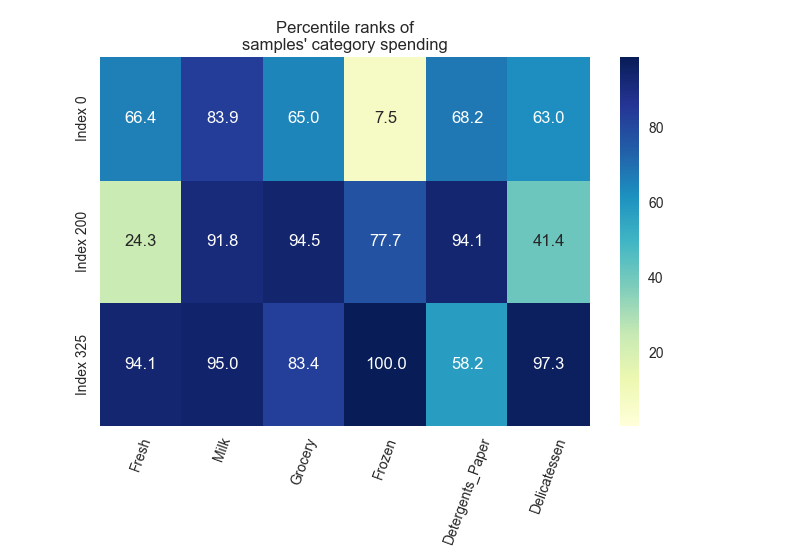
\includegraphics[width=0.9\textwidth]{figures/percentileRanksSampleSpending}
    \label{percentileRanksSampleSpending}
    
    \caption{\textbf{Percentile ranks of samples' category spending. }}
\end{figure}


\section*{Feature Relevance}
Let's figure out if it's possible to determine whether customers purchasing some amount of one category of products will necessarily purchase some proportional amount of another category of products? 

To do this, we can train a supervised regression learner on a subset of the data with one feature removed, and then score how well that model can predict the removed feature.

We predicted the impact of the feature \texttt{Grocery} on customers' spending habits. The prediction score was 0.682 out of 1. This score which tends towards being high indicates that it this feature is not necessary for identifying customers' spending habits. The reason is as follows: 
\begin {itemize}
\item when customers spend on \texttt{Grocery} they also spend on other features, which means we can't decipher spending habits. 
\end{itemize}
What would be better is to regress on a feature that has a \textbf{low} $R^2$ score indicating low correlation.


To get a better understanding of the dataset, we can construct a scatter matrix of each of the six product features present in the data. From figure \ref{scatterplot} we can see that the data for these features is not normally distributed. Its skewed to the right and has a long tail.
\begin{figure}[!hbtp]
\centering
   
    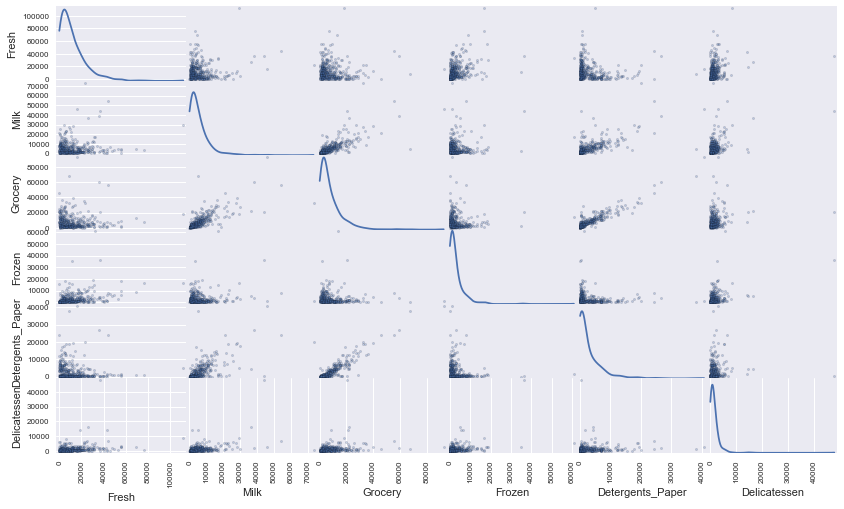
\includegraphics[width=0.9\textwidth]{figures/scatterplot}
    \label{scatterplot}
    
    \caption{\textbf{A scatter matrix for each pair of features in the data. }}
\end{figure}

The pairs \texttt{Grocery} and \texttt{Detergents\_Paper} have a very strong correlation. From the scatterplot, one can see that the data for these two features looks like it could fit a nice diagonal. To formalize my intuition, I performed a pearson's correlation on these two features and got a 0.92 score, noting that a score of 1 is the highest a correlation can be.

Another pair was \texttt{Grocery} and \texttt{Milk}. From the scatterplot, you can kind of see a trending along the diagonal. It had a correlation score of 0.73.

Another pair was \texttt{Milk} and \texttt{Detergents\_Paper}, the pair had a correlation score of 0.66. This confirms my suspicions that \texttt{Grocery} is **not** a strong predictor of overall client spending habits.




\section*{Outlier detection}
The algorithm that we will be using to cluster the data points, \texttt{KMeans} is \emph{very sensitive} to outliers. Since this algorithm uses the distance from the centroids of the clusters, i.e. the means to calculate which data points belong to what cluster, leaving values that are very far off from the rest will influence the structure, leading to undesirable clusters.

As part of the data exploration process, we were careful to analyze the data for potential outliers. We used Tukey's Method for identfying outliers to clean the data. We removed 42 data points from our dataset which corresponds to 10\% of the dataset. In this case we still have around 390 uniques data points for a problem with 6 variables. 


%----------------------------------------------------------------------------------------
%  CHAPTER 
%----------------------------------------------------------------------------------------
\chapter*{Methodology}

\section*{Feature Transformation}
We scaled the data to a more normal distribution and  removed outliers. We then applied PCA to the data to discover which dimensions about the data best maximize the variance of features involved. 

\begin{figure}[!hbtp]
\centering
    
    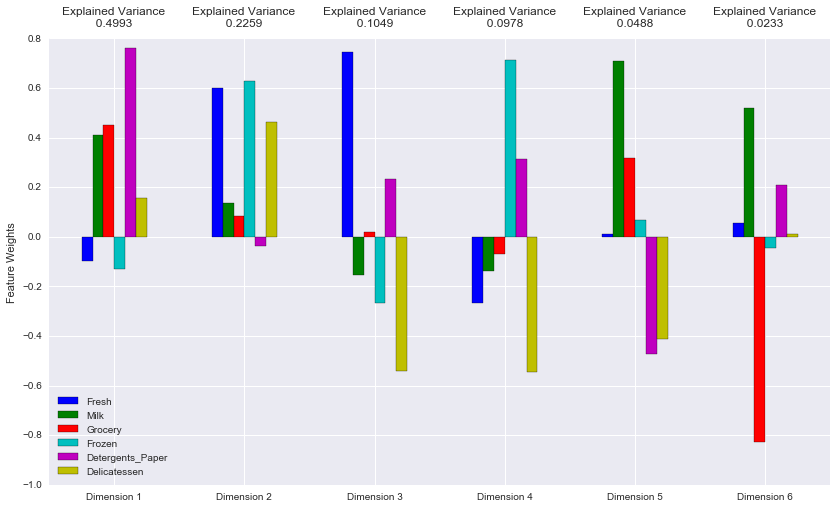
\includegraphics[width=0.9\textwidth]{figures/pca}
    \label{pca}
    
    \caption{\textbf{PCA on the log transformed data. }}
\end{figure}

\begin{figure}[!hbtp]
\centering
    
    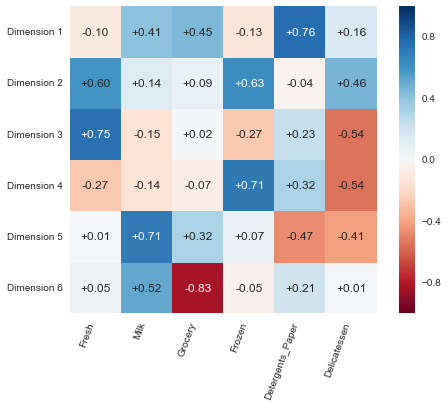
\includegraphics[width=0.9\textwidth]{figures/pcaCorrelation}
    \label{pcaCorrelation}
    
    \caption{\textbf{Correlations on the PCA log transformed data. }}
\end{figure}


Unsurprisingly, dimensions 1 and 2 account for almost 72\% of the variance in the data. One of the interesting aspects of PCA is that the most interesting dynamics occur only in the first $k$ dimension, and then they fall off. In this case, I would say the first \emph{3} components highlight some clear customer segments.    

The first four principal components account for 93\% of the variance in the dataset. For this analysis, we have decided that a correlation value above 0.5+- is deemed significant. 

\begin{itemize}

\item First Principal Component Analysis - Dimension 1 \\
The first principal component is made up of large positive weights in \texttt{Detergents\_Paper}, and lesser but still sizable positive weights on \texttt{Grocery} and \texttt{Milk}. It also correlates with a decrease in \texttt{Fresh} and \texttt{Frozen}. This might represent spending in household staples products that are purchased together. 

It is important to note that we have a lot of variance in customer spending in the correlated features of \texttt{Detergents\_Paper}, \texttt{Grocery} and \texttt{Milk} -- some customers buy more while other customers buy less in these three categories.

\item Second Principal Component Analysis - Dimension 2\\
The second principal component is made up of large positive weights in \texttt{Fresh} and \texttt{Frozen}, a lesser but still sizable weight on \texttt{Delicatessen}, and smaller weights on \texttt{Milk} and \texttt{Grocery}. It also correlates with a slight decrease in \texttt{Detergent\_Paper}. This might represent spending in food items that are purchased together.

\item Third Principal Component Analysis - Dimension 3\\
The third principal component is made up of a large positive weight in \texttt{Fresh}, a small positive weight in \texttt{Detergents\_Paper}, and a significantly lesser positive weight in \texttt{Grocery}. Also, the third principal component has a large negative weight in \texttt{Delicatessen} and a lesser negative weights in \texttt{Milk} and \texttt{Frozen} categories. This might represent spending more in the \texttt{Fresh} category while spending less in \texttt{Delicatessen} category.

We have some variance in customer spending in the correlated features of \texttt{Fresh}, \texttt{Detergents\_Paper} and \texttt{Grocery} -- some customers buy more while other customers buy less in these 3 categories.


\item Fourth Principal Component Analysis - Dimension 4\\
The fourth principal component is made up of a large positive weight in \texttt{Frozen} and a lesser but somewhat sizable positive weight in \texttt{Detergents\_Paper}. Also, this principal component has large negative weight in \texttt{Delicatessen}, a smaller negative weight in \texttt{Fresh}, \texttt{Milk}, and a significantly smaller negative weight in \texttt{Grocery}. This might represent spending more on non-perishable products while simultaneously spending less on perishable products.
\end{itemize}

The first dimension seems to represent customers who spend \emph{significantly} on \texttt{Detergents\_Paper}, spend okay on \texttt{Milk} and \texttt{Grocery}, and none to less on \texttt{Fresh} produce and \texttt{Frozen} products. Another way to understand these first four dimensions is that they each represent a \emph{customer segment}

\section*{Implementation}

Because the first two dimension represent a vast amount of explained variance in the data, we reduced the dataset down to those dimensions. We then performed clustering on the reduced dataset. 

For clustering, we selected the \textbf{KMeans} algorithm for the following reasons:
\begin{itemize} 
\item We want to have a clear delineation of who the various customer segments are. KMeans gives hard partitions and will allow for this.  
\item KMeans scales and is a simple and efficient algorithm unlike the Gaussian Mixture Model which does not scale. If we ever grow the dataset, this difference will save a lot of time in the future.  
\item Easy to understand and compute
\item It's efficient. The time requirement is $O(I*K*m*n)$ as long as the number of clusters is significantly less than m.
  \begin{itemize} 
    \item where $I$ is the number of iterations required for convergence
    \item where $K$ is the number of clusters
    \item where $m$ the number of points
    \item where $n$ is the number of attributes
    \end{itemize}  
\end{itemize} 

Another algorithm we considered was the Gaussian Mixture Model. Which allows for soft-classification, i.e., data point can belong to more than one cluster with probabilities.
   

We calculated the mean silhouette coefficient for the data points and determined that the optimal number of clusters to use in describing the data was two. 

\begin{figure}[!hbtp]
\centering
    
    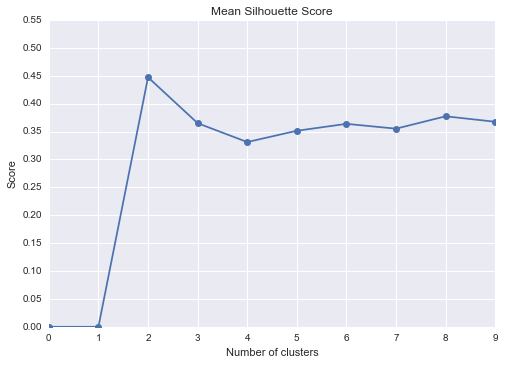
\includegraphics[width=0.9\textwidth]{figures/meanSilhouetteScore}
    \label{meanSilhouetteScore}
    
    \caption{\textbf{The mean silhouette coefficient score for several hypothetical clusters.}}
\end{figure}

%----------------------------------------------------------------------------------------
%  CHAPTER 
%----------------------------------------------------------------------------------------

\chapter*{Results}
(approximately 2 - 3 pages)


\section*{Model Evaluation and Validation}
In this section, the final model and any supporting qualities should be evaluated in detail. It should be clear how the final model was derived and why this model was chosen. In addition, some type of analysis should be used to validate the robustness of this model and its solution, such as manipulating the input data or environment to see how the model’s solution is affected (this is called sensitivity analysis). Questions to ask yourself when writing this section:
\begin{itemize}% 
\item Is the final model reasonable and aligning with solution expectations? Are the final parameters of the model appropriate?
\item Has the final model been tested with various inputs to evaluate whether the model generalizes well to unseen data?
\item Is the model robust enough for the problem? Do small perturbations (changes) in training data or the input space greatly affect the results?
\item Can results found from the model be trusted?
\end{itemize}

\section*{Justification}
In this section, your model’s final solution and its results should be compared to the benchmark you established earlier in the project using some type of statistical analysis. You should also justify whether these results and the solution are significant enough to have solved the problem posed in the project. Questions to ask yourself when writing this section:
\begin{itemize}% 
\item Are the final results found stronger than the benchmark result reported earlier?
\item Have you thoroughly analyzed and discussed the final solution?
\item Is the final solution significant enough to have solved the problem?
\end{itemize}

%----------------------------------------------------------------------------------------
%  CHAPTER 
%----------------------------------------------------------------------------------------

\chapter*{Conclusion}
(approximately 1 - 2 pages)

\section*{Free-Form Visualization}
In this section, you will need to provide some form of visualization that emphasizes an important quality about the project. It is much more free-form, but should reasonably support a significant result or characteristic about the problem that you want to discuss. Questions to ask yourself when writing this section:
\begin{itemize}% 
\item Have you visualized a relevant or important quality about the problem, dataset, input data, or results?
\item Is the visualization thoroughly analyzed and discussed?
\item If a plot is provided, are the axes, title, and datum clearly defined?
\end{itemize}


\section*{Reflection}
In this section, you will summarize the entire end-to-end problem solution and discuss one or two particular aspects of the project you found interesting or difficult. You are expected to reflect on the project as a whole to show that you have a firm understanding of the entire process employed in your work. Questions to ask yourself when writing this section:
\begin{itemize}% 
\item Have you thoroughly summarized the entire process you used for this project?
\item Were there any interesting aspects of the project?
\item Were there any difficult aspects of the project?
\item Does the final model and solution fit your expectations for the problem, and should it be used in a general setting to solve these types of problems?
\end{itemize}

\section*{Improvement}
In this section, you will need to provide discussion as to how one aspect of the implementation you designed could be improved. As an example, consider ways your implementation can be made more general, and what would need to be modified. You do not need to make this improvement, but the potential solutions resulting from these changes are considered and compared/contrasted to your current solution. Questions to ask yourself when writing this section:
\begin{itemize}% 
\item Are there further improvements that could be made on the algorithms or techniques you used in this project?
\item Were there algorithms or techniques you researched that you did not know how to implement, but would consider using if you knew how?
\item If you used your final solution as the new benchmark, do you think an even better solution exists?
\end{itemize}



\end{document}  